\documentclass[10pt,xcolor={dvipsnames}, aspectratio=169]{beamer}
\usetheme[
%%% option passed to the outer theme
%    progressstyle=fixedCircCnt,   % fixedCircCnt, movingCircCnt (moving is deault)
  ]{Feather}
  
% If you want to change the colors of the various elements in the theme, edit and uncomment the following lines

% Change the bar colors:
\setbeamercolor{Feather}{fg=NavyBlue!20,bg=NavyBlue}

% Change the color of the structural elements:
\setbeamercolor{structure}{fg=NavyBlue}

% Change the frame title text color:
\setbeamercolor{frametitle}{fg=black!5}

% Change the normal text colors:
\setbeamercolor{normal text}{fg=black!75,bg=gray!5}

%% Change the block title colors
\setbeamercolor{block title}{use=Feather,bg=Feather.fg, fg=black!90} 


% Change the logo in the upper right circle:
%\renewcommand{\logofile}{example-grid-100x100pt} 
%% This is an image that comes with the LaTeX installation
% Adjust scale of the logo w.r.t. the circle; default is 0.875
% \renewcommand{\logoscale}{0.55}

% Change the background image on the title and final page.
% It stretches to fill the entire frame!
% \renewcommand{\backgroundfile}{example-grid-100x100pt}

%-------------------------------------------------------
% INCLUDE PACKAGES
%-------------------------------------------------------

\usepackage[utf8]{inputenc}
\usepackage[utf8]{vietnam}
\usepackage[english]{babel}
\usepackage[T1]{fontenc}
\usepackage{amsmath}
% \usepackage{helvet}

%% Load different font packages to use different fonts
%% e.g. using Linux Libertine, Linux Biolinum and Inconsolata
% \usepackage{libertine}
% \usepackage{zi4}

%% e.g. using Carlito and Caladea
\usepackage{carlito}
\usepackage{caladea}
\usepackage{zi4}

%% e.g. using Venturis ADF Serif and Sans
% \usepackage{venturis}

%-------------------------------------------------------
% DEFFINING AND REDEFINING COMMANDS
%-------------------------------------------------------

% colored hyperlinks
\newcommand{\chref}[2]{
  \href{#1}{{\usebeamercolor[bg]{Feather}#2}}
}

%-------------------------------------------------------
% INFORMATION IN THE TITLE PAGE
%-------------------------------------------------------

\title[] % [] is optional - is placed on the bottom of the sidebar on every slide
{ % is placed on the title page
      \textbf{Task Scheduling In Real-time System}
}

\subtitle[Task Scheduling Algorithm Selection]
{
      \textbf{}
}

\author[Quang Khanh]
{      Quang Khanh \\
      {\ttfamily khanh.tq170083@gmail.com}
}

\institute[]
{%
      Hanoi University of Science and Technology\\
	  School of Information and Communication Technology
}

\date{\today}

%-------------------------------------------------------
% THE BODY OF THE PRESENTATION
%-------------------------------------------------------

\begin{document}

%-------------------------------------------------------
% THE TITLEPAGE
%-------------------------------------------------------

{\1% % this is the name of the PDF file for the background
\begin{frame}[plain,noframenumbering] % the plain option removes the header from the title page, noframenumbering removes the numbering of this frame only
  \titlepage % call the title page information from above
\end{frame}}


\begin{frame}{Content}{}
\tableofcontents
\end{frame}

\section{Problem Statement}

\begin{frame}{Entities in the Task-Scheduling Problems}
	\begin{block}
	{Cluster of machines}
	Cloud computing is built over a group of machines in order to provide services to users.
	\end{block}
	
	\begin{figure}
		\centering
		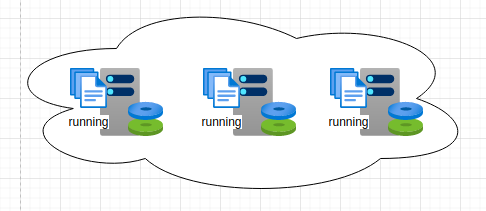
\includegraphics[scale=0.7]{images/system.png}
		\caption{Virtual machines}
	\end{figure}
\end{frame}

\begin{frame}{Entities in the Task-Scheduling Problems}
	\begin{block}
	{Tasks}
	Users submit tasks at random time to the cloud by API web services.
	\end{block}
	\begin{block}
	{Notice}
	Users submitting tasks is a stochastic process.
	\end{block}
	\begin{figure}
		\centering
		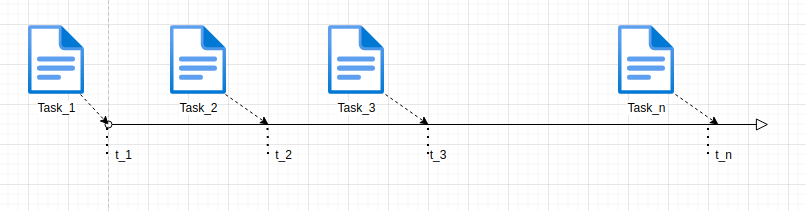
\includegraphics[scale=0.4]{images/task_arrivals.png}
		\caption{Task arrivals}
	\end{figure}
	
\end{frame}

\begin{frame}
{Workflow of task scheduling}
	\begin{columns}[T] % align columns
		\begin{column}{.4\textwidth}
			\begin{block}
			{The order of task scheduling process} 
				\begin{itemize}
					\item Users submit tasks to the datacenter. 
					\item Tasks are dispatched to waiting-queue. 
					\item Scheduling finds matched VM for each task in waiting-queue.
				\end{itemize}
			\end{block}
	\end{column}%
	\hfill%
	\begin{column}{.56\textwidth}
		\begin{figure}
			\centering
			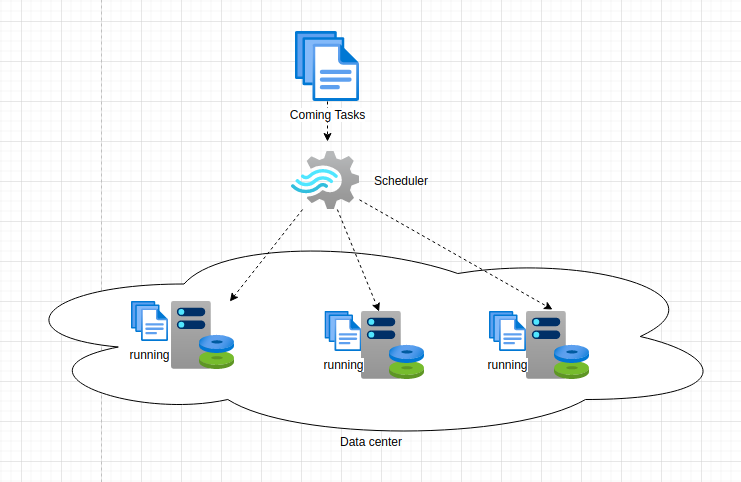
\includegraphics[scale=0.4]{images/coming_tasks.png}
			\caption{tasks are scheduled}
		\end{figure}
	\end{column}%
	\end{columns}
\end{frame}

\begin{frame}
{Workflow of task scheduling}
	\begin{columns}[T] % align columns
		\begin{column}{.4\textwidth}
			\begin{block}
			{The order of task scheduling process} 
				\begin{itemize}
					\item Users submit tasks to the datacenter. 
					\item Tasks are dispatched to waiting-queue. 
					\item Scheduling finds matched VM for each task in waiting-queue.
					\item Tasks are dispatched to matched VMs.
				\end{itemize}
			\end{block}
	\end{column}%
	\hfill%
	\begin{column}{.56\textwidth}
		\begin{figure}
			\centering
			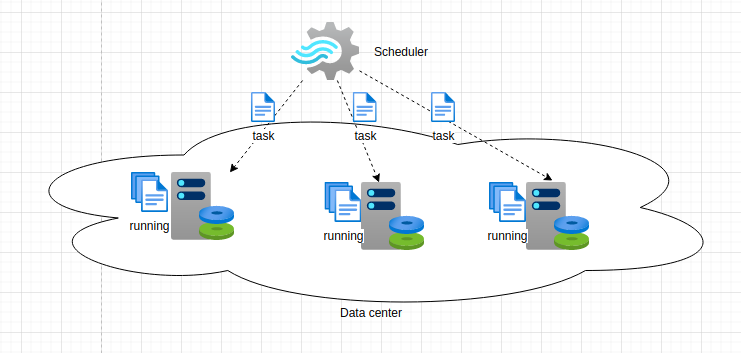
\includegraphics[scale=0.4]{images/dispatching.png}
			\caption{tasks are dispatched}
		\end{figure}
	\end{column}%
	\end{columns}
\end{frame}

\begin{frame}
{Mathematical Model}
	\begin{columns}[T] % align columns
		\begin{column}{.48\textwidth}
			\begin{block}
				{Task i}
				\begin{itemize}
					\item cpu\_request(i): quantities of cpu unit
					\item cpu\_cores\_request(i): number requested cores of cpu
					\item ram\_request(i)
					\item disk\_request(i)
					\item priority(i)
				\end{itemize}
			\end{block}
	\end{column}%
	\hfill%
	\begin{column}{.48\textwidth}
		\begin{block}
		{VM j}
			\begin{itemize}
				\item Cpu(j)
				\item Cpu\_cores(j)
				\item Mips(j)
				\item Ram(j)
				\item Disk(j)
			\end{itemize}
		\end{block}
	\end{column}%
	\end{columns}
\end{frame}

\begin{frame}
	{Mathematical Model}
	\begin{block}
		{Waiting queue}
		$Q = \{T_{i}, ..., T_{j}\}$ is the set of waiting tasks
	\end{block}
	\begin{block}
		{Trace} 
		Trace(i, j) = 1 if task i is matched with machine j
	\end{block}
	\begin{block}
		{Running queue}
		$R(M) = \{T_{x_{1}}, ..., T_{x_{k}}\}$ is a set of running tasks on the virtual machine M
	\end{block}
	\begin{block}
		{Defered tasks} 
		Defered(i, j) = 1 if task i is running in machine j then instantly cancelled.
	\end{block}
\end{frame}

\begin{frame}
	{Mathematical Model}
	\begin{block}
		{Avialable resources of virtual machine j}
		$A\_cpu(j) = Cpu(j) - \sum_{i \in R(j)}{cpu\_request(i)} * (1 - Defered(i, j))$\\ 
		$A\_ram(j) = Ram(j) - \sum_{i \in R(j)}{ram\_request(i)} * (1 - Defered(i, j))$ \\ 
		$A\_disk(j) = Disk(j) - \sum_{i \in R(j)}{disk\_request(i)} * (1 - Defered(i, j))$ \\ 
	\end{block}
\end{frame}

\begin{frame}
	{Mathematical Model}
	\begin{block}
		{Constraints} 
		\begin{center}
			$\forall$ j = 1, ..., $N_{M},$
		\end{center}
		\begin{equation*}
			\sum_{i = 1}^{N_{T}}{Trace[i, j] * cpu\_request(i)} < A\_cpu(j)
		\end{equation*}
		\begin{equation*}
			\sum_{i = 1}^{N_{T}}{Trace[i, j] * ram\_request(i)} < A\_ram(j)
		\end{equation*}
		\begin{equation*}
			\sum_{i = 1}^{N_{T}}{Trace[i, j] * disk\_request(i)} < A\_disk(j)
		\end{equation*}
	\end{block}
\end{frame}

\begin{frame}
	{Mathematical Model}
	\begin{block}
		{Priority constraint}
		$\forall i = 1, ..., N_{T}$
		\begin{equation*}
			priority(i) > 6 \implies \sum_{j = 1}^{N_{M}}{Defered(i, j)} = 0
		\end{equation*}
	\end{block}
\end{frame}

\begin{frame}
	{Objectives}
	\begin{block}
	{Defered Rate} 
	Minimize 
	\begin{center}
		$\frac{\sum_{i, j}{Defered(i, j)}}{N_{T}}$	
	\end{center}
	\end{block}
	
	\begin{block}
	{Make-span}
	The time from tasks are submitted to all tasks are completed
	\end{block}	
\end{frame}

\begin{frame}
	{Problems} 
	\begin{block}
		{Instructions} 
		Cannot estimate the total instructions of a task. 
	\end{block}
	
	\begin{block}
		{Machines' state}
		Cannot estimate the states of all machines in the next time step, which leads to ineffective scheduling-plan.
	\end{block}
\end{frame}

\begin{frame}
	{Proposal}
	\begin{block}
	{To solve the problems} 
	We need a strategy to estimate status of a task after its duration
	\end{block}
	
	\begin{block}
		{Correlated features} 
		Features correlated to the status of a task include: 
		\begin{itemize}
			\item cpu\_request
			\item ram\_request
			\item MIPS of the machine in which it's executed
			\item duration
		\end{itemize}
	\end{block}
\end{frame}


{\1
\begin{frame}[plain,noframenumbering]
  \finalpage{Thank you for listening!}
\end{frame}}

\end{document}